{\descr{Обчислити площу плоскої фігури, обмеженою данними лініями}}

$$
  y=\dfrac{2}{x^2-1},{\qquad} y = 2-x
$$


\begin{figure}[h!]
  \centering
  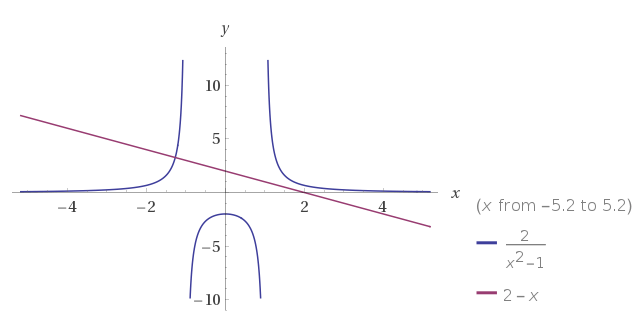
\includegraphics[width=14cm]{rozrahunkova_02/04_01.png}
  \label{fig:rr_02_04_01}
  \centering
\end{figure}

Судячи з графіку, задані лінії мають лише 1 точку пересічення $(\dfrac{2}{x^2-1} = 2-x)$, тому будемо вважати що таку площу знайти неможливо, оскільки вона нічим не обмежена.
